% Бүлэг 1

\chapter{Багшийн журнал вэб системийн хөгжүүлэлт судалгааны хэсэг} 
% Бүлгийн нэр
\label{Chapter1} % Энэ бүлэг рүү ишлэл хийх бол \ref{Chapter1} командыг ашигла 

%-------------------------------------------------------------------------------

% Агуулгад ашигласан хэвшүүлэлтийн зарим командын тодорхойлолт
\newcommand{\keyword}[1]{\textbf{#1}}
\newcommand{\tabhead}[1]{\textbf{#1}}
\newcommand{\code}[1]{\texttt{#1}}
\newcommand{\file}[1]{\texttt{\bfseries#1}}
\newcommand{\option}[1]{\texttt{\itshape#1}}

%-------------------------------------------------------------------------------

\section{Хэрэглэгчийн судалгаа}
Энэхүү дипломын ажлын хүрээнд журнал дээр хийсэн судалгааг 2017 оны 09-р сарын 25-с 2017 оны 10-р сарын 23-ны өдөр хүртэл хийсэн судалгаа.
%-------------------------------------------------------------------------------
\begin{figure}[htbp]
	\centering
	
\includegraphics[scale=0.05]{figures/20171006_161409.jpg}
	\centering
	
\includegraphics[scale=0.05]{figures/20171006_162113.jpg}
	\centering
	
\includegraphics[scale=0.05]{figures/20171006_162422.jpg}
	\caption[Хэрэглэгчийн судалгаа]{Сургууль дээр хэвлэгдэж ирдэг дэвтэр,журнал.}
	%\label{fig:Chart1}
\end{figure}

\begin{itemize}
\item Анги удирдсан багшийн дэвтэр(IV-XII анги)
\item Багшийн журнал (I-III анги)
\item Багшийн журнал (IV-XII анги)
\end{itemize}
	
\begin{enumerate}
	\item Анги удирдсан багшийн дэвтэр(IV-XII анги)
	\begin{enumerate}
		\item[1.1] Нүүр /1 нүүр/
		\item[1.2] Товьёг /1 нүүр/
		\item[1.3] Хуанли /1 нүүр/
		\item[1.4] Хичээлийн хуваарь /1 нүүр/
		\item[1.5] Журнал хөтлөх заавар /1 нүүр/
		\item[1.6] Суралцагчийн дэлгэрэнгүй бүртгэл /4 нүүр/
		\item[1.7] Хичээлээс гадуурх ажилд суралцагчийн оролцоо /4 нүүр/
		\item[1.8] Дугуйлан, секцэд хамрагдаж буй байдал /2 нүүр/
		\item[1.9] Суралцагчийн ололт амжилт /2 нүүр/
		\item[1.10] Эрүүл, зөв дадал хэвшил төлөвшүүлэх ажлын тэмдэглэл /4 нүүр/
		\item[1.11] Суралцагчийн төлөвшилд гарч буй өөрчлөлтийн талаарх тэмдэглэл /2 нүүр/
		\item[1.12] Багш, эцэг эхийн хамтын ажиллагаа /2 нүүр/
		\item[1.13] Сурах бичгийн бүртгэл /2 нүүр/
		\item[1.14] Ирцийн бүртгэл /8 нүүр/
		\item[1.15] Үнэлгээ 4 улирлаар /8 нүүр/
		\item[1.16] Жилийн эцсийн үнэлгээ /2 нүүр/
		\item[1.17] Шалгалтын дүн /1 нүүр/
		\item[1.18] Шилжилт хөдөлгөөн / Тасарсан хичээлийн цагийн тооцоо /1 нүүр/
		\item[1.19] Анги удирдсан багшийн тэмдэглэл /1 нүүр/\\ 
		\begin{flushright}
			{\large \textbf{ Нийт: 24 хуудас}}
		\end{flushright}
	\end{enumerate}
	\item Багшийн журнал (I-III анги)
	\begin{enumerate}
		\item[2.1] Нүүр /1 нүүр/
		\item[2.2] Товьёг /1 нүүр/
		\item[2.3] Хуанли /1 нүүр/
		\item[2.4] Хичээлийн хуваарь /1 нүүр/
		\item[2.5] Журнал хөтлөх заавар /1 нүүр/
		\item[2.6] Ирцийн бүртгэл /8 нүүр/
		\item[2.7] Үнэлгээ /86 нүүр/
		\item[2.8] Багшийн тэмдэглэл /86 нүүр/
		\item[2.9] Багшийн тэмдэглэл /1 нүүр/
		\item Анги удирдсан багшийн дэвтэр(I-III анги)
		\item[2.10] Нүүр /1 нүүр/
		\item[2.11] Товьёг /1 нүүр/
		\item[2.12] Журнал хөтлөх заавар /1 нүүр/
		\item[2.13] Суралцагчийн дэлгэрэнгүй бүртгэл /4 нүүр/
		\item[2.14] Хичээлээс гадуурх ажилд суралцагчийн оролцоо /4 нүүр/
		\item[2.15] Дугуйлан, секцэд хамрагдаж буй байдал /2 нүүр/
		\item[2.16] Суралцагчийн ололт амжилт /2 нүүр/
		\item[2.17] Эрүүл, зөв дадал хэвшил төлөвшүүлэх ажлын тэмдэглэл /4 нүүр/
		\item[2.18] Суралцагчийн төлөвшилд гарч буй өөрчлөлтийн талаарх тэмдэглэл /2 нүүр/
		\item[2.19] Багш, эцэг эхийн хамтын ажиллагаа /2 нүүр/
		\item[2.20] Сурах бичгийн бүртгэл /2 нүүр/
		\item[2.21] Шилжилт хөдөлгөөн / Тасарсан хичээлийн цагийн тооцоо /1 нүүр/
		\item[2.22] Анги удирдсан багшийн тэмдэглэл /1 нүүр/\\ 
		\begin{flushright}
			{\large \textbf{ Нийт: 65 хуудас}}
		\end{flushright}
	\end{enumerate}
	\item Багшийн журнал (IV-XII анги)
	\begin{enumerate}
		\item[2.1] Нүүр /1 нүүр/
		\item[2.2] Товьёг /1 нүүр/
		\item[2.3] Хуанли /1 нүүр/
		\item[2.4] Хичээлийн хуваарь /1 нүүр/
		\item[2.5] Журнал хөтлөх заавар /1 нүүр/
		\item[2.6] Ирц үнэлгээ /120 нүүр/
		\item[2.7] Багшийн тэмдэглэл /120 нүүр/
		\item[2.8] {Багшийн тэмдэглэл /1 нүүр/} \hfill \break
		\begin{flushright}
			{\large \textbf{ Нийт: 64 хуудас}}
		\end{flushright}
	\end{enumerate}
\end{enumerate}
%-------------------------------------------------------------------------------
%\section{}
Уг судалгааг Монгени цогцолбор сургууль, Ирээдүй цогцолбор 81-р сургууль, Сэтгэмж цогцолбор сургууль дээр хийгдсэн бөгөөд судалгааны явцад гарсан үр дүн дунджаар тавигдсан болно.
\begin{figure}[htbp]
	\centering
	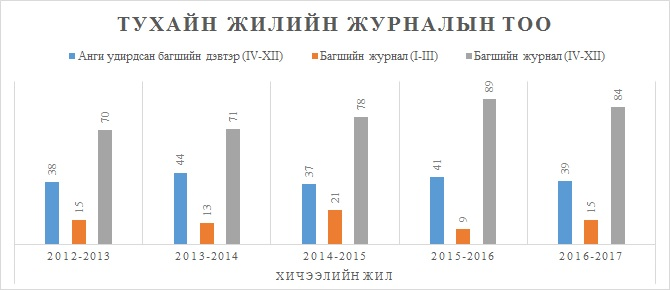
\includegraphics[scale=0.8]{Chart/Chart1}
	\caption[Хэрэглэгчийн судалгаа]{2012-2017 оны хичээлийн жил тус бүрд нэг сургуульд дунджаар хэвлэгдэж ирэх журналын тоо(Судалгаа)}
	\label{fig:Chart2}
\end{figure}
\begin{figure}[htbp]
	\centering
	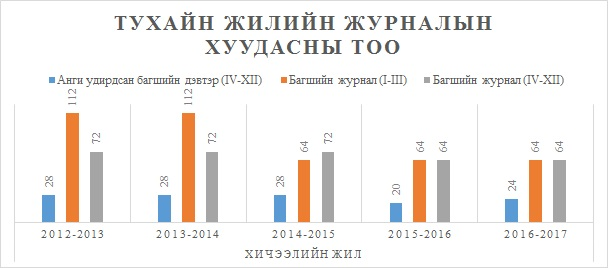
\includegraphics[scale=0.8]{Chart/Chart2}
	\caption[Хэрэглэгчийн судалгаа]{2012-2017 оны хичээлийн жил тус бүрд хэвлэгдсэн журнал, дэвтрийн хуудасны тоо (Судалгаа)}
	\label{fig:Chart2}
\end{figure}
\begin{figure}[htbp]
	\centering
	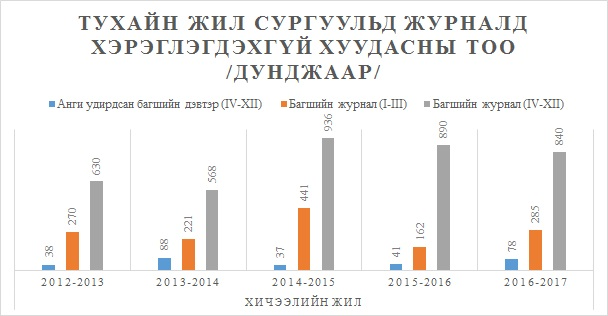
\includegraphics[scale=0.8]{Chart/Chart3}
	\caption[Хэрэглэгчийн судалгаа]{2012-2017 оны хичээлийн жил тус бүрд хэрэглэгдээгүй хуудасны тоо (Судалгаа)}
	\label{fig:Chart2}
\end{figure}\begin{figure}[htbp]
\centering
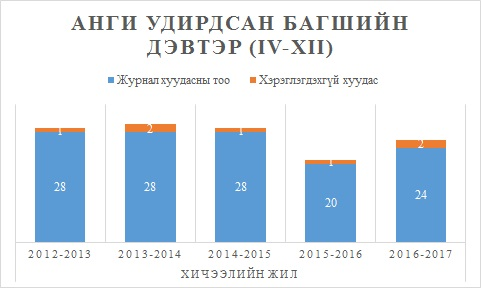
\includegraphics[scale=1]{Chart/Chart4}
\caption[Хэрэглэгчийн судалгаа]{2012-2017 оны хичээлийн жил тус бүрд нэг сургуульд Анги удирдсан багшийн дэвтэр(IV-XII)-ийн хэрэглэгдсэн, хэрэглэгдээгүй хуудасны тоо (Судалгаа)}
\label{fig:Chart2}
\end{figure}\begin{figure}[htbp]
\centering
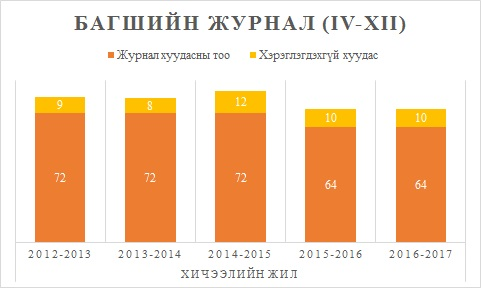
\includegraphics[scale=1]{Chart/Chart5}
\caption[Хэрэглэгчийн судалгаа]{2012-2017 оны хичээлийн жил тус бүрд нэг сургуульд Багшийн журнал(IV-XII)-ийн хэрэглэгдсэн, хэрэглэгдээгүй хуудасны тоо (Судалгаа)}
\label{fig:Chart2}
\end{figure}\begin{figure}[htbp]
\centering
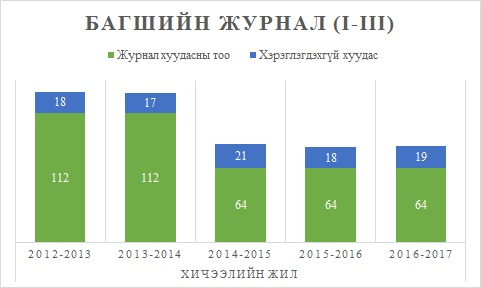
\includegraphics[scale=1]{Chart/Chart6}
\caption[Хэрэглэгчийн судалгаа]{2012-2017 оны хичээлийн жил тус бүрд нэг сургуульд Багшийн журнал (I-III)-ийн хэрэглэгдсэн, хэрэглэгдээгүй хуудасны тоо (Судалгаа)}
\label{fig:Chart2}
\end{figure}\begin{figure}[htbp]
\centering
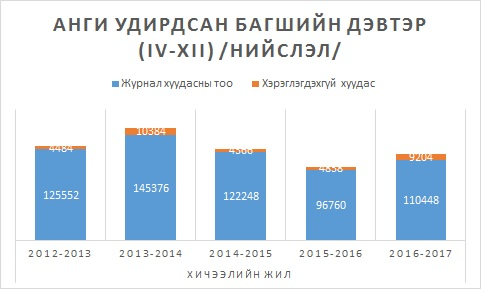
\includegraphics[scale=0.9]{Chart/Chart7}
\caption[Хэрэглэгчийн судалгаа]{2012-2017 оны хичээлийн жил тус бүрд Нийслэлийн хэмжээнд Анги удирдсан багшийн дэвтэр(IV-XII)-ийн хэрэглэгдсэн, хэрэглэгдээгүй хуудасны тоо (Судалгаа)}
\label{fig:Chart2}
\end{figure}\begin{figure}[htbp]
\centering
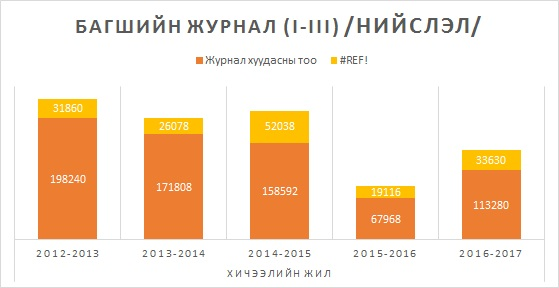
\includegraphics[scale=0.9]{Chart/Chart8}
\caption[Хэрэглэгчийн судалгаа]{2012-2017 оны хичээлийн жил тус бүрд Нийслэлийн хэмжээнд Багшийн журнал (I-III)-ийн хэрэглэгдсэн, хэрэглэгдээгүй хуудасны тоо (Судалгаа)}
\label{fig:Chart2}
\end{figure}\begin{figure}[htbp]
\centering
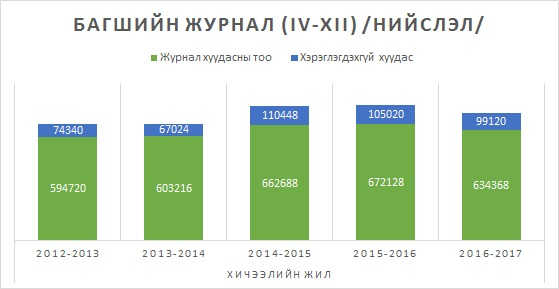
\includegraphics[scale=0.9]{Chart/Chart9}
\caption[Хэрэглэгчийн судалгаа]{2012-2017 оны хичээлийн жил тус бүрд Нийслэлийн хэмжээнд Багшийн журнал(IV-XII)-ийн хэрэглэгдсэн, хэрэглэгдээгүй хуудасны тоо (Судалгаа)}
\label{fig:Chart2}
\end{figure}\begin{figure}[htbp]
\centering
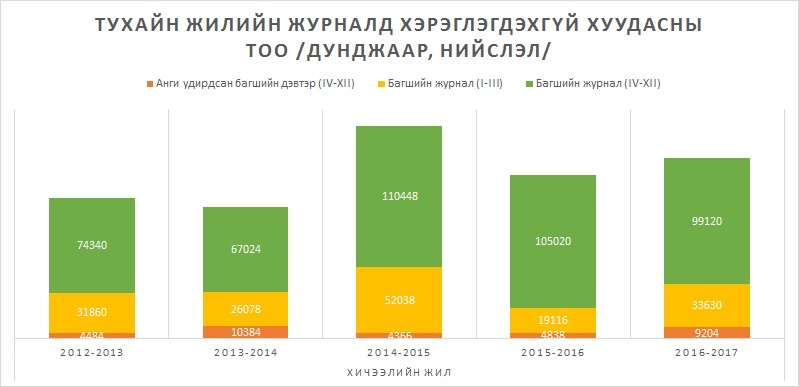
\includegraphics[scale=0.7]{Chart/Chart10}
\caption[Хэрэглэгчийн судалгаа]{2012-2017 оны хичээлийн жил тус бүрд Нийслэлийн хэмжээнд хэрэглэгдээгүй хуудасны тоо(Судалгаа)}
\label{fig:Chart2}
\end{figure}
\section{Судалгааны дүгнэлт}
Энэхүү судалгааны үр дүнд хэрэглэгдээгүй цаасны хэмжээ 650000 орчим гарсан бөгөөд багшийн журнал 5 жил, Анги удирдсан багшийн дэвтэр 20 жилийн хугацаанд хэрэглэгдэн цахим болж устгагддаг байна. Одоогийн байдлаар програм хангамжийн байгууллагууд төрөл бүрийн цахим журнал хийж байгаа боловч бүрэн орлож чадахгүй байна. Иймд зөвхөн журнал гэдэг зүйлийг дангаар авч үзэж цахимжуулах арга хэмжээ авах хэрэгтэй.\\
500 ширхэг бичгийн цаас хийхэд дунджаар 2,6 кг мод хэрэглэгддэг бол Нийслэлийн хэмжээнд нийт сургуулиудын хэмжээнд 3,3 тонн цаас хий дэмий үрэгддэг гэсэн үг юм. 
%-------------------------------------------------------------------------------

\section{Технологийн судалгаа}

\section{MySQL}
MySQL нь холбоост өгөгдлийн санг удирдах систем юм. MySQL хэмээх нэрний хувьд уг системийг санаачлан хөгжүүлэгч Micheal Widenius-ын охины нэр My + SQL(Structed Query Language) гэсэн утгатай ажээ.
Энэ систем нь GNU (General Public License) буюу нээлтэй эхийн систем учир хүссэн хэн бүхэн хөгжүүлэлтэнд оролцож, үнэгүй хэрэглэж болох юм. Эзэмшигч нь алдарт Java-г хөгжүүлсэн Sun MicroSystems компани байсан ба, одоогоор Sun-г Oracle корпораци эзэмших болсон билээ.
Үнэгүй програм хангамжийн өгөгдлийн санг удирдах системд ихэвчлэн MySQL-ийг хэрэглэдэг бөгөөд тэдгээрийн сонгодог жишээ гэвэл Joomla, Drupal, Wordpress, phpBB гэх мэт агуулга удирдах системүүд (CMS-Content Management System), Wikipedia, Facebook, Google гэх мэт томоохон компаниуд хэрэглэдэг юм.
Хөгжүүлэлт нь C/C++ хэл дээр хийгдсэн ба AIX, BSDi, FreeBSD, HP-UX, i5/OS, Linux, Mac OS X, NetBSD, Novell NetWare, OpenBSD, OpenSolaris, eComStation, OS/2 Warp, QNX, IRIX, Solaris, Symbian, SunOS, SCO OpenServer, SCO UnixWare, Sanos, Tru64, Microsoft Windows гэсэн олон үйлдлийн системүүд дээр ажилладаг.
MySQL бол хамгийн өргөн хэрэглээтэй нээлттэй эхийн (Open Source) өгөгдлийн сан удирдах програм юм. Анх 1995 онд зах зээлд гарсан ба с/с++ хэл дээр бичигдсэн. Одоогийн байдлаар 5.7 нь хамгийн сүүлийн хувилбар болон гараад байна. Энэ сүүлийн хувилбар дээр нэмэгдсэн давуу талууд гэвэл 3 дахин хурдан үйл ажиллагаатай болсон мөн натив JSON дэмжигчтэй болсон гэх мэт шинэлэг үйлдлүүд нэмэгдсэн байна.

\section{Php}
  Rasmus Lerdorf WWW-д вэб хуудас үүсгэх үедээ өгөгдөл боловсруулах хялбархан арга хайж байгаад 1995 онд PHP хэлийг скрипт хэл байдлаар зохиосон.
PHP нь сервер талын скрипт хэл ба динамик вэб хуудас хийхэд илүү тохиромжтой. Энэ скрипт хэл нь энгийн хэрэглээний вэб сайтаас эхлээд байгууллагын иж бүрэн вэб программ хийж болохоор MySQL мэтийн өгөгдлийн сантай харилцан ажиллах боломжтой.
Хуудас ачаалах үед броузерээр нэг бүрчлэн уншдаг HTML-тэй адилгүй, PHP баримтыг бэлтгэхдээ серверээр урьдчилан боловсруулдаг. PHP код агуулсан хуудас нь хэрэглэгчийн броузерт илгээгдхээс өмнө серверээр боловсруулагдсан байдаг.
PHP хэлний өөр нэг давуу тал бол скриптэн хэл юм. Ихэнх програмчлалын хэлнүүдэд ажиллахын өмнө машины хэл рүү хөрвүүлэх тусгай файлууд /compile/ шаардлагатай байдаг бол PHP хэлний хувьд хөрвүүлэлт хийх шаардлагагүй байдаг тул код засварлах болон шалгахад илүү хурдан байдаг

\section{JQuery}
2006 оны эхээр АНУ-ын Нью-Иорк хотын BarCamp-д John Resig хэмээх вэб хөгжүүлэгч залуу jQuery сангийн тухай анх мэдэгджээ. Resig өөрийн вэб сайтдаа: Тухайн үед байгаа сангуудад сэтгэл дундуур байгаагаа, мөн түүнчлэн JavaScript – ий тухай бичилтийг нь багасгаснаар маш их ажил хөнгөвчлөх боломжтой, энгийн үйлдлүүдэд зориулан тусгай хэрэгслүүд нэмэх хэрэгтэй гэж дурдсан байдаг.
Хөгжүүлэх нийгэмлэгт jQuery нь томоохон амжилт авчирсан төдийгүй улмаар маш хурдтай хөгжсөн. Бусад хөгжүүлэгчид сан боловсронгуй болгоход тусалж эхэлснээр jQuery – гийн анхны хувилбар 1.0 нь 2006 оны 8-р сарын 26- нд гарсан.
Түүнээс хойш jQuery 3.1.1 хувилбар гарсан ба хөгжүүлэлтийн нийгэмлэгээс plug-in –ийг маш ихээр оруулсан. Plug-in нь jQuery – ийн сангийн цөм хэсэг биш харин нэмэлт хэрэгсэл юм. 
jQuery – гийн давуу талууд нь:
\begin{itemize}
\item Файлын хэмжээ бага
\item Маш энгийн бичилттэй
\item Холбоо бүхий method – уудтай
\item Санг өргөтгөх plug-in нь энгийн бүтэцтэй
\item Асар том онлайн нийгэмлэгтэй
\item JQueryUI мэтийн jQuery – гийн нэмэлт сонголтуудтай
\end{itemize}
\section{Service}
2006 оны эхээр АНУ-ын Нью-Иорк хотын BarCamp-д John Resig хэмээх вэб хөгжүүлэгч залуу jQuery сангийн тухай анх мэдэгджээ. Resig өөрийн вэб сайтдаа: Тухайн үед байгаа сангуудад сэтгэл дундуур байгаагаа, мөн түүнчлэн JavaScript – ий тухай бичилтийг нь багасгаснаар маш их ажил хөнгөвчлөх боломжтой, энгийн үйлдлүүдэд зориулан тусгай хэрэгслүүд нэмэх хэрэгтэй гэж дурдсан байдаг.
Хөгжүүлэх нийгэмлэгт jQuery нь томоохон амжилт авчирсан төдийгүй улмаар маш хурдтай хөгжсөн. Бусад хөгжүүлэгчид сан боловсронгуй болгоход тусалж эхэлснээр jQuery – гийн анхны хувилбар 1.0 нь 2006 оны 8-р сарын 26- нд гарсан.
Түүнээс хойш jQuery 3.1.1 хувилбар гарсан ба хөгжүүлэлтийн нийгэмлэгээс plug-in –ийг маш ихээр оруулсан. Plug-in нь jQuery – ийн сангийн цөм хэсэг биш харин нэмэлт хэрэгсэл юм. 
jQuery – гийн давуу талууд нь:
\begin{itemize}
\item Файлын хэмжээ бага
\item Маш энгийн бичилттэй
\item Холбоо бүхий method – уудтай
\item Санг өргөтгөх plug-in нь энгийн бүтэцтэй
\item Асар том онлайн нийгэмлэгтэй
\item JQueryUI мэтийн jQuery – гийн нэмэлт сонголтуудтай
\end{itemize}
\section{Бүлгийн дүгнэлт}
%-------------------------------------------------------------------------------